\documentclass[tikz,border=2mm]{standalone}
\tikzset
{% \x = angle, \h=wave height, \n=wave number
   declare function={wave(\x,\h,\n)=1+\h*sin(\n*\x-90*(\n-1));}
}
\begin{document}
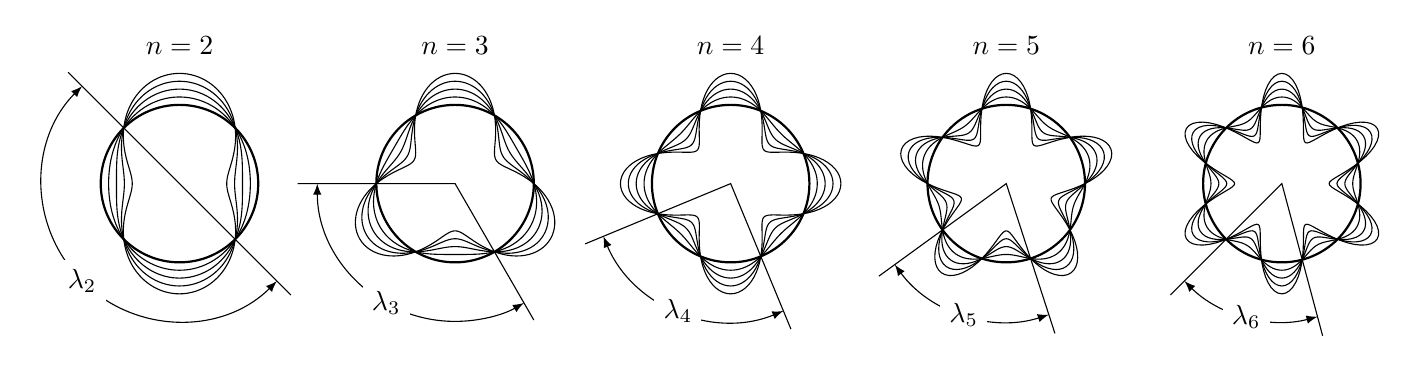
\begin{tikzpicture}
\foreach\i in {2,...,6}
{
  \begin{scope}[shift={(3.5*\i,0)}]
    \node at (0,1.75) {$n=\i$};
    \draw[thick] (0,0) circle (1);
    \foreach\j in {0.1,0.2,0.3,0.4}
      \draw plot[domain=0:360,samples=181] ({wave(\x,\j,\i)*cos(\x)},{wave(\x,\j,\i)*sin(\x)});
   \pgfmathsetmacro\sa{-90+90*(4*\i-3)/\i} % start angle
   \pgfmathsetmacro\ea{\sa+360/\i}         % end angle
   \draw (\sa:2) -- (0,0) -- (\ea:2);
   \draw[latex-latex] (\sa:1.75) arc (\sa:\ea:1.75) node[midway,fill=white] {$\lambda_\i$};
   \end{scope}
}
\end{tikzpicture}
\end{document}